\chapter{Limitación de recursos}
\minitoc
\clearpage

\section{Introdución}

A limitación dos recursos físicos é unha cuestión crítica no referente á seguridade do sistema, xa que un contedor malicioso podería facer uso exhaustivo dos mesmos, chegando a ocupar a práctica totalidade destes e prexudicando así a outros contedores aloxados na mesma máquina, ou mesmamente á propia máquina anfitrioa, podéndose producir así un ataque de denegación de servizo (\gls{DoS}) \cite{OS-level-security}. Numerosos aspectos deben ser tidos en conta para asegurar a seguridade integral do sistema no referente á utilización adecuada dos recursos físicos. Dividiremos o estudo en: CPU, memoria, disco e rede.\\

Analizaremos as diferentes respostas a este tipo de sobreempregas de recursos, tentando facer unha comparativa entre execucións debidamente controladas e outras que non o estarán, para o cal empregaranse pequenas aplicacións contedorizadas.

\section{Modelo de limitación de recursos de Docker}

Docker relega algunha das súas funcionalidades de seguridade directamente nas características inherentes do \textit{kernel} de GNU/Linux. Polo tanto, o límite dos privilexios entre os contedores e a máquina anfitrioa xa foi deseñado. Os controis técnicos que levan este límite inclúen o illamento de procesos mediante os espazos de nomes (\textit{namespaces}\footnote{http://man7.org/linux/man-pages/man7/namespaces.7.html}), permitindo así illar usuarios, procesos, redes ou dispositivos, e administración dos recursos mediante \textit{cgroups}\footnote{http://man7.org/linux/man-pages/man7/cgroups.7.html}. Ambos, espazos de nomes e \textit{cgroups}, fusionáronse a partir da versión 2.6.24 do \textit{kernel} de GNU/Linux. Deste xeito, os contedores Docker execútanse baixo un suposto entorno illado e controlado na máquina anfitrioa. No referente aos límites de recursos, tema principal desta sección, debemos pór a nosa atención nos \textit{cgroups}, posto que o seu obxectivo é precisamente que un proceso non tome todos os recursos dispoñíbeis do sistema. Isto inclúe os recursos partillados de CPU, memoria, ancho de banda da rede e E/S de disco \cite{To-Docker-Or-Not-To-Docker}. \\

Debido a estas delegacións de seguridade sobre os \textit{cgroups}, non debemos influír na súa funcionalidade (e polo tanto no control de seguridade que realiza) con opcións de Docker como pode ser o \textit{flag --privileged}, que eleva as capacidades do contedor e elimina tamén as limitacións impostas polos \textit{cgroups} \cite{state-of-art-docker-security}, deixando ao sistema vulnerábel. É dicir, Docker posúe opcións avanzadas que permiten outorgar dun maior número de privilexios aos seus contedores, evadindo os controis realizados polos \textit{cgroups}, por exemplo; mais estas opcións poden supor un gran risco para o noso sistema e debémolas evitar sempre que nos sexa posíbel.\\

A mellora de seguridade aportada pola axuda dos \textit{cgroups} e do espazo de nomes non deixa de mellorar cada día, polo que resulta importante manter as tecnoloxías de contedorización actualizadas para obter as últimas correccións de seguridade. Por exemplo, até a versión 1.10 de Docker, non existía un espazo de nomes para o usuario, o que pode ser considerado un risco crítico. Se un proceso conseguise dalgunha forma ``rachar'' o contedor e saír del, executándose na máquina anfitrioa, ao non existir un espazo de nomes para os usuarios, o proceso obtería os mesmos privilexios que tiña dentro do contedor, mais na máquina anfitrioa. Polo tanto, se o proceso tiña privilexios de superusuario (\gls{UID}=0) no interior do contedor, tamén gañaría privilexios de superusuario no exterior, podendo modificar o sistema a pracer. Produciríase entón un ataque de escalada de privilexios, no que un usuario non autorizado obtería privilexios sobre o sistema aos que non debería ter acceso. Aínda que as posibilidades de que isto suceda son moi poucas, non debe ser considerado coma algo insignificante.\\

Como xa foi comentado, a partir da versión 1.10 de Docker os espazos de nomes dos usuarios foron tidos en conta, supondo unha das actualizacións de seguridade máis importantes desta tecnoloxía de contedorización. Dende dita versión, cada proceso posúe o seu propio conxunto de identificadores para usuarios e grupos. Por exemplo, se un proceso dentro do contedor posúe o \gls{UID} 0, pertencente ao superusuario, na máquina anfitrioa podería estar mapado a un \gls{UID} calquera, como por exemplo o 3000, pertencente a un usuario non privilexiado. Este mapado evita que procesos executados dentro dun contedor poidan obter permisos de superusuario fóra do contedor. \cite{state-of-art-docker-security} \\

Non obstante, debemos configurar o noso sistema con moita cautela, posto que aínda que dende a versión 1.10 estes espazos de nomes foros introducidos en Docker, dita característica está dispoñíbel, mais non está activada por defecto \cite{docker-security}. É labor do administrador do sistema asegurar a súa correcta configuración e seguridade. Para isto, pode facer emprega de ferramentas de auditoría como a descrita na sección \ref{DockerBeckAuditTool}.

\section{Modelo de limitación de recursos de Singularity}
\label{modeloLimitacionRecursosSingularity}

A diferenza de Docker, o modelo de funcionamento dos contedores Singularity entende que a limitación de recursos queda fóra da súa xurisdición, posto que os contedores Singularity foron deseñados para correr como calquera outra aplicación do sistema. É dicir, os procesos poden ser observados dende fóra do contedor e, polo tanto, xestionados por ferramentas externas como calquera outro proceso do sistema. Polo tanto, enténdese que estas limitacións deben ser xestionadas por un administrador de recursos propio do sistema \cite{singularity-limits}; idea que cobra máis sentido se temos en conta que son un tipo de contedores creados especialmente para o seu uso en \gls{HPC}.\\

Tendo en conta o marco de traballo no que este proxecto se desenvolve, no cal se estuda a seguridade en entornos \gls{HPC}/\textit{Cloud} nas infraestruturas do \gls{CESGA}, poden ser aproveitadas funcionalidades xa implantadas no sistema para a repartición e limitación dos recursos. Deste xeito, o xestor da carga de traballo para \gls{HPC} empregado nestes momentos no centro é Slurm, tal e como foi explicado na sección \ref{infraestruturaSlurm}. Así, a meirande parte das tarefas de distribución da carga de traballo, e polo tanto de asegurar a limitación dos recursos físicos, dependen deste xestor.

\section{CPU e memoria}

Estes dous recursos físicos foron xuntados nunha soa sección posto que a súa forma de control e limitación faise dun xeito practicamente idéntico, presentando soamente diferenzas dependendo da tecnoloxía de contedorización a empregar.

\subsection{Docker}

Grazas á delegación nos \textit{cgroups}, Docker posúe a funcionalidade de poder limitar a cantidade de memoria que cada contedor pode empregar, evitando así que un contedor ocupe toda a memoria e deixe sen recursos a outros contedores, ou peor aínda, á propia máquina anfitrioa \cite{state-of-art-docker-security}. Do mesmo xeito, a CPU tamén é controlada polos \textit{cgroups}, baixo a mesma premisa.

\subsubsection{Probas de limitación de CPU e memoria con Docker}

Para a realización das probas de memoria, escribiuse un sinxelo código en C, dispoñíbel no anexo \ref{consumidorMemoria}, cuxa lóxica baséase nun bucle infinito de reservas dinámicas de memoria, sen facer liberación da mesma. Tras pór a proba dito código, observouse que o contedor era parado automaticamente polo sistema. Isto resultou ser porque, por defecto, Docker conta cunha ferramenta de prevención de \textit{out-of-memory} (\gls{OOM}). É dicir, se os límites son superados, o sistema encargarase de matar pola súa conta aos procesos. De non querer que isto suceda, deberiamos activar o \textit{flag} \textit{--oom-kill-disable} cando lanzamos un contedor Docker. Obviamente, esta medida resultaría contraproducente contra a defensa de un ataque de \gls{DoS}, polo que debemos evitar empregala sempre que poidamos.\\

Neste caso, para poder facer uso do pequeno código de proba, desactivaremos esta opción. Para a realización da proba, crearemos un contedor Docker con límites de memoria e CPU, que serán xestionados polos \textit{cgroups}. Cando lanzamos o programa xa compilado, coa opción de de \gls{OOM} desactivada, podemos ver como a memoria e a utilización da CPU axústanse aos límites outorgados no momento de invocación do contedor. A forma de invocar ao contedor só permite a emprega de 1.5 de CPU e de 500 MB de memoria.

\begin{lstlisting}[,caption={Emprega de límites de CPU e memoria en contedores Docker}]
docker run --memory=500m --cpus="1.5" --oom-kill-disable -it ubuntu /bin/bash
\end{lstlisting}

Para a comprobación dos cumprimento dos límites establecidos empregouse a ferramenta \textit{Docker Stats}\footnote{\url{https://docs.docker.com/engine/reference/commandline/stats/}}, tal e como pode ser observado na figura \ref{MemoriaFull}. Tamén se comprobou que a emprega de CPU por parte da máquina anfitrioa non superaba os límites, tal e como amosa a figura \ref{CPUDocker}.

\begin{figure}[]
\centerline{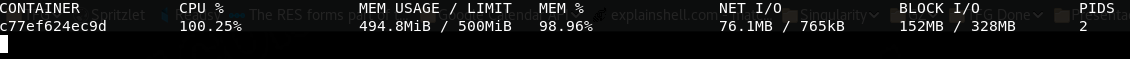
\includegraphics[width=15cm]{figuras/MemoriaFull.png}}
\caption{Emprega total de CPU e memoria dun contedor Docker con límites}
\label{MemoriaFull}
\end{figure}

\begin{figure}[]
\centerline{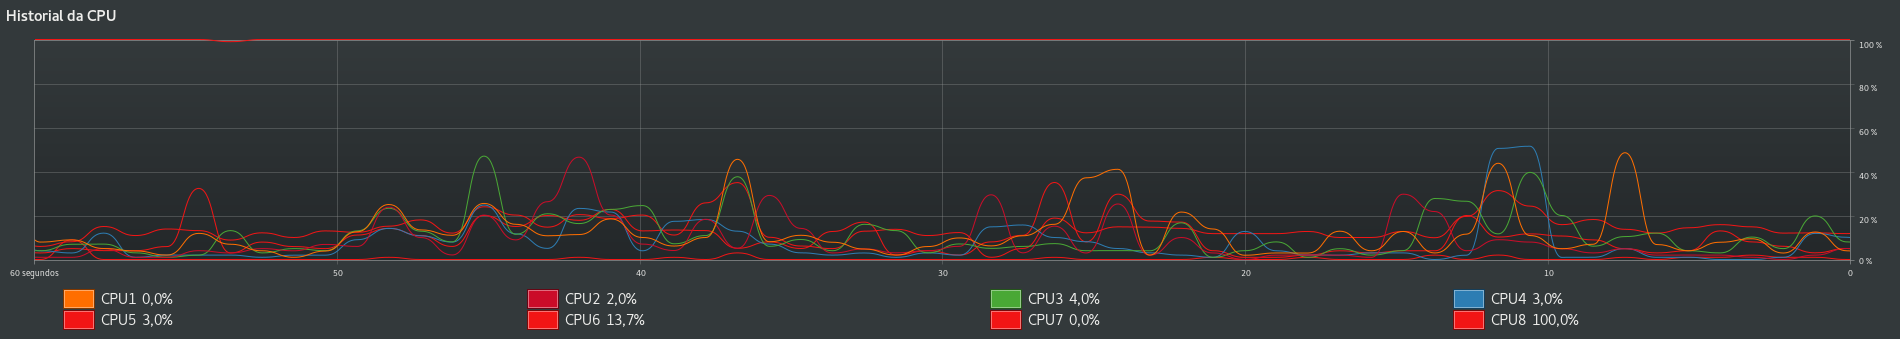
\includegraphics[width=15cm]{figuras/CPUDocker.png}}
\caption{Revisión da CPU empregada na máquina anfitrioa}
\label{CPUDocker}
\end{figure}

\subsection{Singularity}

Tal e como foi explicado na sección \ref{modeloLimitacionRecursosSingularity}, Singularity entende que non é a súa xurisdición o control dos recursos do sistema, ao estar deseñado para correr como unha aplicación máis do sistema. Deste xeito, neste caso, CPU e memoria son dous dos factores claramente controlados polo xestor de recursos Slurm. Así, á hora de lanzar un proceso con este xestor, empregando comandos como {\it srun} ou {\it sbatch}, podemos indicar \textit{flags} que indiquen con exactitude os recursos dos que queremos facer uso. Abstraéndonos do proceso, Slurm encargarase de que o usuario non poida superar os límites que solicitou. Por exemplo, algunhas das opcións máis amplamente empregadas e que dan solución ao problema dos límites de recursos son:

\begin{itemize}
    \item \textbf{\textit{-N} ou \textit{--nodes}:} solicita o mínimo número de nodos que deben ser reservados para certo traballo. Tamén é posíbel indicar o máximo número de nodos. No caso de indicar soamente un número, ese indicará o mínimo e o máximo. No caso de non haber nodos suficientes para o traballo indicado nese momento, o traballo acadará un estado de ``pendente'', á espera de que os nodos precisos sexan liberados.
    \item \textbf{\textit{-n} ou \textit{--ntasks}:} indica o número máximo de tarefas a desenvolver e fornece os recursos suficientes. O valor predeterminado é dunha tarefa por cada nodo.
    \item \textbf{\textit{--ntasks-per-core}:} pensado para ser executado en combinación coa opción {\it --ntasks}, indica o número máximo de tarefas a ser executadas por cada núcleo.
    \item \textbf{\textit{--ntasks-per-node}:} indica o número de tarefas a ser desenvolvidas por cada nodo. De ser empregado xunto coa opción {\it --ntasks}, devandita opción terá prioridade no canto desta.
    \item \textbf{\textit{--mem}:} indica a memoria \gls{RAM} que poderá obter cada nodo. Se facemos especificación dun tamaño de memoria igual a cero, tratarase como un caso especial e outorgarase a ese traballo toda a memoria dispoñíbel de cada nodo. Ter en conta que se traballamos cun \textit{cluster} heteroxéneo, o límite de memoria virá dado polo nodo cun tamaño de memoria máis pequeno.
    \item \textbf{\textit{--mem-per-cpu}:} indica a memoria \gls{RAM} que será preciso asignar por cada CPU. Destacar que as opcións {\it --mem-per-cpu} e {\it --mem} son mutuamente exclusivas.
\end{itemize}

\section{Disco}

Cando falamos das limitacións a ter en conta no referente á emprega de disco, debemos discernir dous casos diferenciados. O primeiro deles fai referencia á E/S, posto que un contedor que faga amplo uso deste factor podería ter un impacto prexudicial noutros contedores ou na mesma máquina anfitrioa. O segundo caso fai referencia á emprega de disco no que ten que ver coa súa capacidade.\\

Por exemplo, cando se empregan algúns dos controladores de almacenamento como pode ser \textit{aufs}, Docker non limita a emprega de disco dos contedores. Un contedor cun volume de almacenamento pode encher este volume e afectar a outros contedores na mesma máquina anfitrioa, ou incluso á mesma, se o almacenamento especificado na ruta ``{\it /var/lib/docker}'' non está montado nunha partición separada \cite{To-Docker-Or-Not-To-Docker}.

\subsection{Cotas de disco}
\label{quotas}

Para evitar que un contedor empregue a totalidade ou meirande parte do disco, impedindo a correcta execución doutros, cómpre aplicar políticas de limitación no uso do mesmo. Estas políticas poden ser aplicadas doadamente coa emprega de cotas, permitindo establecer diversidade de límites en función dos usuarios do sistema.\\

Grazas a este feito, os contedores Singularity quedarán perfectamente limitados no referente á utilización do disco. Pola súa contra, os contedores Docker, posto que son controlados polo demo Docker con permisos de superusuario, non se verán limitados, xa que o superusuario terá a capacidade {\it CAP\_SYS\_RESOURCE}\footnote{\url{http://man7.org/linux/man-pages/man7/capabilities.7.html}} activada, a cal permite ignorar os límites de cotas de disco, entre outras cousas.\\

Para comprobar este feito, realizouse unha proba de concepto dentro dunha máquina virtual Ubuntu Xenial 16.04, na que se estableceron cotas de disco para un determinado usuario e posteriormente tentouse escribir un ficheiro que superase as limitacións establecidas, facendo uso de contedores baseados en Alpine Linux 3.7.0 (que presentan a característica de que o seu sistema base está deseñado para ocupar só 4-5MB , excluíndo o \textit{kernel}). As limitacións escollidas foron de 10MB \textit{soft} e de 100MB \textit{hard}. O proceso de aplicación destas cotas pode ser consultado no apéndice \ref{scriptQuotas}.

\subsubsection{Probas de cotas nun contedor Docker}

\begin{lstlisting}[,caption={Escritura en disco excedendo cuota máxima en contedor Docker}]
nuevousuariocuotas@localhost:~$ docker run -ti alpine
/home # dd if=/dev/zero of=fichero bs=200M count=1
1+0 records in
1+0 records out

#Saimos do contedor
nuevousuariocuotas@localhost:~$ docker ps -s 
CONTAINER ID        IMAGE               COMMAND             CREATED             STATUS              PORTS               NAMES               SIZE
1aba32e99ce5        alpine              "/bin/sh"           4 minutes ago       Up 3 seconds                            gifted_bohr         210MB (virtual 214MB)
\end{lstlisting}

No caso do contedor executado baixo a tecnoloxía de Docker, a escritura é posíbel e os límites son superados. Se ao rematar comprobamos o tamaño actual do contedor, pódese ver coma ocupa un total de 210MB, superando así a cota total de disco establecida para o usuario.\\

\subsubsection{Probas de cotas nun contedor Singularity}

\begin{lstlisting}[,caption={Escritura en disco excedendo cuota máxima en contedor Singularity}]
dd if=/dev/zero of=fichero bs=200M count=1
dd: error writing 'fichero': Disk quota exceeded
1+0 records in
0+0 records out
102354944 bytes (102 MB, 98 MiB) copied, 0.701354 s, 146 MB/s
\end{lstlisting}

Como se pode ver, as cotas entran en xogo no caso dos contedores Singularity, impedindo a escritura de ficheiros unha vez o límite máximo é excedido.\\

\subsubsection{Alternativa a aplicar en Docker}

A execución de cotas sobre contedores Docker non resulta efectiva. De todos xeitos, esta tecnoloxía presenta unha xestión sobre os discos máis avanzada, que debe ser estudada con maior detemento.\\

Docker amósanos a posibilidade de almacenar datos no disco dende dúas perspectivas ben diferenciadas:

\begin{enumerate}
    \item \textbf{Almacenamento persistente no disco:} os datos non se perden unha vez remata a execución do contedor.
    \item \textbf{Almacenamento volátil:} os datos soamente son accesíbeis namentres o contedor está executándose.
\end{enumerate}

Para facer esta diferenciación de tipos de almacenamento, Docker presenta varios tipos de montaxe do disco, tal e como pode ser observado na figura \ref{typesOfMountsDocker}. Unha vez dentro do contedor, os datos veranse da mesma forma, no entanto é importante diferencialos para facer un uso adecuado do disco. Así, distinguimos:

\begin{figure}
\centerline{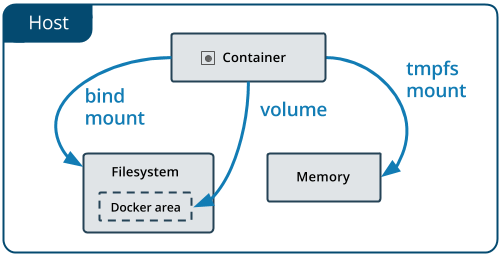
\includegraphics[width=15cm]{figuras/typesOfMountsDocker.png}}
\caption{Tipos de montaxe de disco en Docker}
\small
\centerline{Fonte: \url{https://docs.docker.com/storage/}}
\label{typesOfMountsDocker}
\end{figure}

\begin{enumerate}
    \item \textbf{Volumes}: almacenados nalgunha parte do sistema de ficheiros que será xestionado por Docker. Os procesos non pertencentes a Docker non deberían modificar o seu contido, e é considerada a mellor forma de realizar un almacenamento persistente empregando contedores Docker, xa que posúen a característica de estar illados da propia máquina anfitrioa. Ademais, un mesmo volume pode ser compartido entre varios contedores e son doadamente transportábeis cara outra máquina. O seu tamaño pode ser xestionado mediante comandos propios de Docker, pondo solución así a posíbeis ataques de denegación de servizo.
    \item \textbf{\textit{Bind mounts}}: son a outra forma de almacenamento persistente xestionada por Docker. O seu funcionamento baséase na emprega dun espazo de disco compartido coa propia máquina anfitrioa (polo que procesos externos poderían modificar estes datos). Un efecto secundario deste feito é que é posíbel facer cambios no sistema de ficheiros da máquina anfitrioa con permisos de superusuario, pudendo chegar a modificar ou eliminar datos importantes do sistema. Polo tanto, esta forma de almacenamento ten importantes implicacións de seguridade, incluíndo un posíbel impacto nos procesos do sistema non referentes a Docker.
    \item \textbf{Montaxes \textit{tmpfs}}: supoñen a forma de almacenamento non persistente, gardando os datos soamente de forma temporal no tempo de vida do contedor e non chegando a escribir no sistema de ficheiros da máquina anfitrioa. A emprega deste tipo de montaxes pode ser moi interesante se estamos a facer uso de contedores para despregamentos rápidos e lixeiros, coma podería ser un contedor para probas.
    
    Este tipo de almacenamento presenta a perigosa característica, dende o punto de vista da seguridade informática, de que por defecto non posúe ningún tipo de limitación no espazo de disco que certo contedor poida empregar. En troques, si que é posíbel establecer controis e restrinxir o espazo máximo a empregar dentro de cada contedor, coa limitación de que soamente é factíbel baixo a emprega de certos controladores. Docker admite varios controladores de almacenamento, empregando unha arquitectura conectábel, sendo estes os encargados de como as imaxes e os contedores son almacenados e xestionados polo \textit{host}.
    
    Así, se queremos limitar o espazo, deberemos empregar controladores concretos como pode ser \textit{devicemapper}, un framework baseado no \textit{kernel} de GNU/Linux que sustenta moitas das tecnoloxías avanzadas de xestión de volumes neste tipo de sistemas. Debe ser tido en conta que é precisa unha configuración específica para poder empregar este controlador con Docker que non é admitida por todos os sistemas operativos, polo que o seu uso non resulta trivial. Como dato de interese, destacar que \textit{devicemapper} opera a nivel de bloque, no canto de nivel de arquivo, acadando así un rendemento mellor que coa emprega dun sistema de ficheiros a nivel de sistema operativo.
    
    Para comprender un pouco mellor a complexidade asociada, é preciso entender que a elección dun controlador de disco vén limitado por unha serie de dependencias coma poden ser a edición de Docker, o sistema operativo e mesmamente a distribución do mesmo. Tamén poden ser requiridos paquetes a maiores para a súa instalación. Ademais, algúns controladores precisan dun formato específico do sistema de ficheiros da máquina anfitrioa, polo que de existir requirimentos externos que limiten a elección dun sistema de ficheiros específico, isto podería limitar enormemente as nosas opcións. Deste xeito, amósase unha táboa de configuracións consideradas estábeis nas versións máis recentes dalgúns dos sistemas operativos GNU/Linux máis soados:

% \usepackage{graphicx}
\begin{table}[H]
\centering
\caption{Configuracións de controladores de almacenamento}
\label{conf-controladores-almacenamento}
\resizebox{\textwidth}{!}{%
\begin{tabular}{|c|c|}
\hline
\textbf{Distribución GNU/Linux} & \textbf{Controladores de almacenamento recomendados}\\ \hline
Ubuntu & \textit{aufs}, \textit{devicemapper}, \textit{overlay2}, \textit{overlay}, \textit{zfs}, \textit{vfs}\\ \hline
Debian & \textit{aufs}, \textit{devicemapper}, \textit{overlay2}, \textit{overlay}, \textit{vfs}\\ \hline
CentOS & \textit{devicemapper}, \textit{vfs}\\ \hline
Fedora & \textit{devicemapper}, \textit{overlay2} (experimental), \textit{overlay} (experimental), \textit{vfs}\\ \hline
\end{tabular}%
}
\end{table}
    
    Debemos ter en conta que cada controlador terá algunha vantaxe característica sobre os outros, dependendo da configuración propia de cada sistema. Aínda así, estes aspectos quedan fóra do ámbito do estudo da seguridade, polo que non serán estudados con detemento.
    
    Finalmente, é de vital importancia destacar que se é preciso realizar un cambio nos controladores, os contedores que empregasen o controlador anterior, deixarán de ser accesíbeis, sendo preciso realizar unha parada nos mesmos, exportalos a un medio externo e volver a montalos baixo os novos controladores, o que podería supor unha gran desaceleración do sistema. Polo tanto, é relevante realizar unha adecuada elección do controlador.
    
\end{enumerate}

\section{Rede}
\label{QoSRede}

A limitación da rede supón un caso bastante especial, posto que ningunha das tecnoloxías de contedorización a estudar fai un control especial sobre esta, o que podería levar a posíbeis ataques de denegación de servizo. É por iso que cómpre aplicar políticas externas de calidade de servizo que aseguren un funcionamento correcto da mesma.

\subsection{Enfoque de Docker sobre a rede}

As redes que Docker configura até arestora están pensadas para funcionar baixo unha filosofía do ``mellor esforzo'' para todo o tráfico existente. Isto implica que parámetros tales como o ancho de banda, a fiabilidade ou o número de paquetes por segundo non poden ser garantidos. Consecuencia deste feito, a emprega dunha única aplicación que faga un uso intensivo do ancho de banda da rede podería implicar un pobre ou incluso inaceptábel rendemento para calquera outra aplicación que comparta esa rede.\\

Así, a solución pasa pola emprega da denominada calidade de servizo (\textit{Quality of Service}, \gls{QoS}), unha serie de mecanismos que fornecen un trato preferenciado a diferentes tráficos e aplicacións \cite{dockerQoS}. Noutras verbas, non é Docker o encargado de xestionar os límites de recursos das redes, senón que de quixer, debemos ser nós quen, a través de medios alternativos debemos establecelos.

\subsection{Enfoque de Singularity sobre a rede}

Repetindo a idea, Singularity fai uso directo de moitos dos recursos do sistema, incluída a rede, sendo compartida directamente coa máquina anfitrioa. Non existen mecanismos propios de limitación da rede, senón que debe ser administrada por servizos externos.

\subsection{Solución común: \gls{QoS}}

A \gls{QoS} pode ser entendida coma o rendemento da rede tal e como o percibe o usuario final. Os parámetros de \gls{QoS} abranguen todos os aspectos dunha conexión, sendo particularmente importantes:

\begin{itemize}
\item Tasa de transmisión (ancho de banda)
\item Retardo (latencia)
\item Variación do retardo (\textit{jitter})
\item Perda de paquetes
\end{itemize}

Dentro dos sistemas GNU/Linux, a QoS está presente como parte do subsistema de rede \textit{iproute}\footnote{\url{http://linux-ip.net/articles/Traffic-Control-HOWTO/}}, permitindo repartir o ancho de banda en función de distintos criterios e baseando o control nun sistema de colas. A gran flexibilidade que outorga este sistema será útil para poder facer un control diferenciado da rede segundo as tecnoloxías de contedorización empregadas, posto que como quedou patente, non todas empregan o mesmo modelado.\\

Como caso de estudo, farase uso do comando {\it tc}, pertencente ao subsistema \textit{iproute}.

\subsubsection{Probas de limitación de rede con Docker}

O modelo de rede de Docker, no seu funcionamento por defecto, é dicir en modo \textit{bridge}, crea unha interface de rede que é empregada para realizar a conexión entre os contedores e a propia máquina. Aproveitaremos o feito de que Docker permite a creación de diferentes interfaces de rede para a conexión dun ou múltiples contedores para aplicar regras de limitación do tráfico de rede.\\

Realizarase unha proba de concepto na que se limitará a velocidade do tráfico da rede. Aplicarase unha limitación mediante unha disciplina de colas sen facer uso de clases, seguindo unha lóxica bastante simple. Enténdese que se é posíbel aplicar estas limitacións, tamén será posíbel aplicar limitacións máis complexas, que variarán segundo a necesidade do entorno. Así, aplicarase unha disciplina ``TBF'' (\textit{Token Bucket Filter}), unha das disciplinas sen clases máis empregadas para limitar o tráfico de rede dunha interface, como é o noso caso. Establecerase tamén unha cola de 1024 kbits, permitindo refachos de ata 200 kbits. Os pasos seguidos para establecer estas limitacións poden ser observados no apéndice \ref{scriptQoSDocker}.\\

Para a execución desta proba despregarase un entorno de rede nos servizos de computación na nube do \gls{CESGA}. Dentro deste entorno existirá unha \gls{MV} coa tecnoloxía de Docker instalada sobre a mesma e correndo un contedor sobre o que aplicaremos as limitacións. Para a comprobación das probas, tratarase de enviar un arquivo a outra máquina virtual empregando o protocolo \gls{SFTP}. O esquema seguido pode ser observado na figura \ref{DiagramaQoSRedeDocker}.\\

\begin{figure}
\centerline{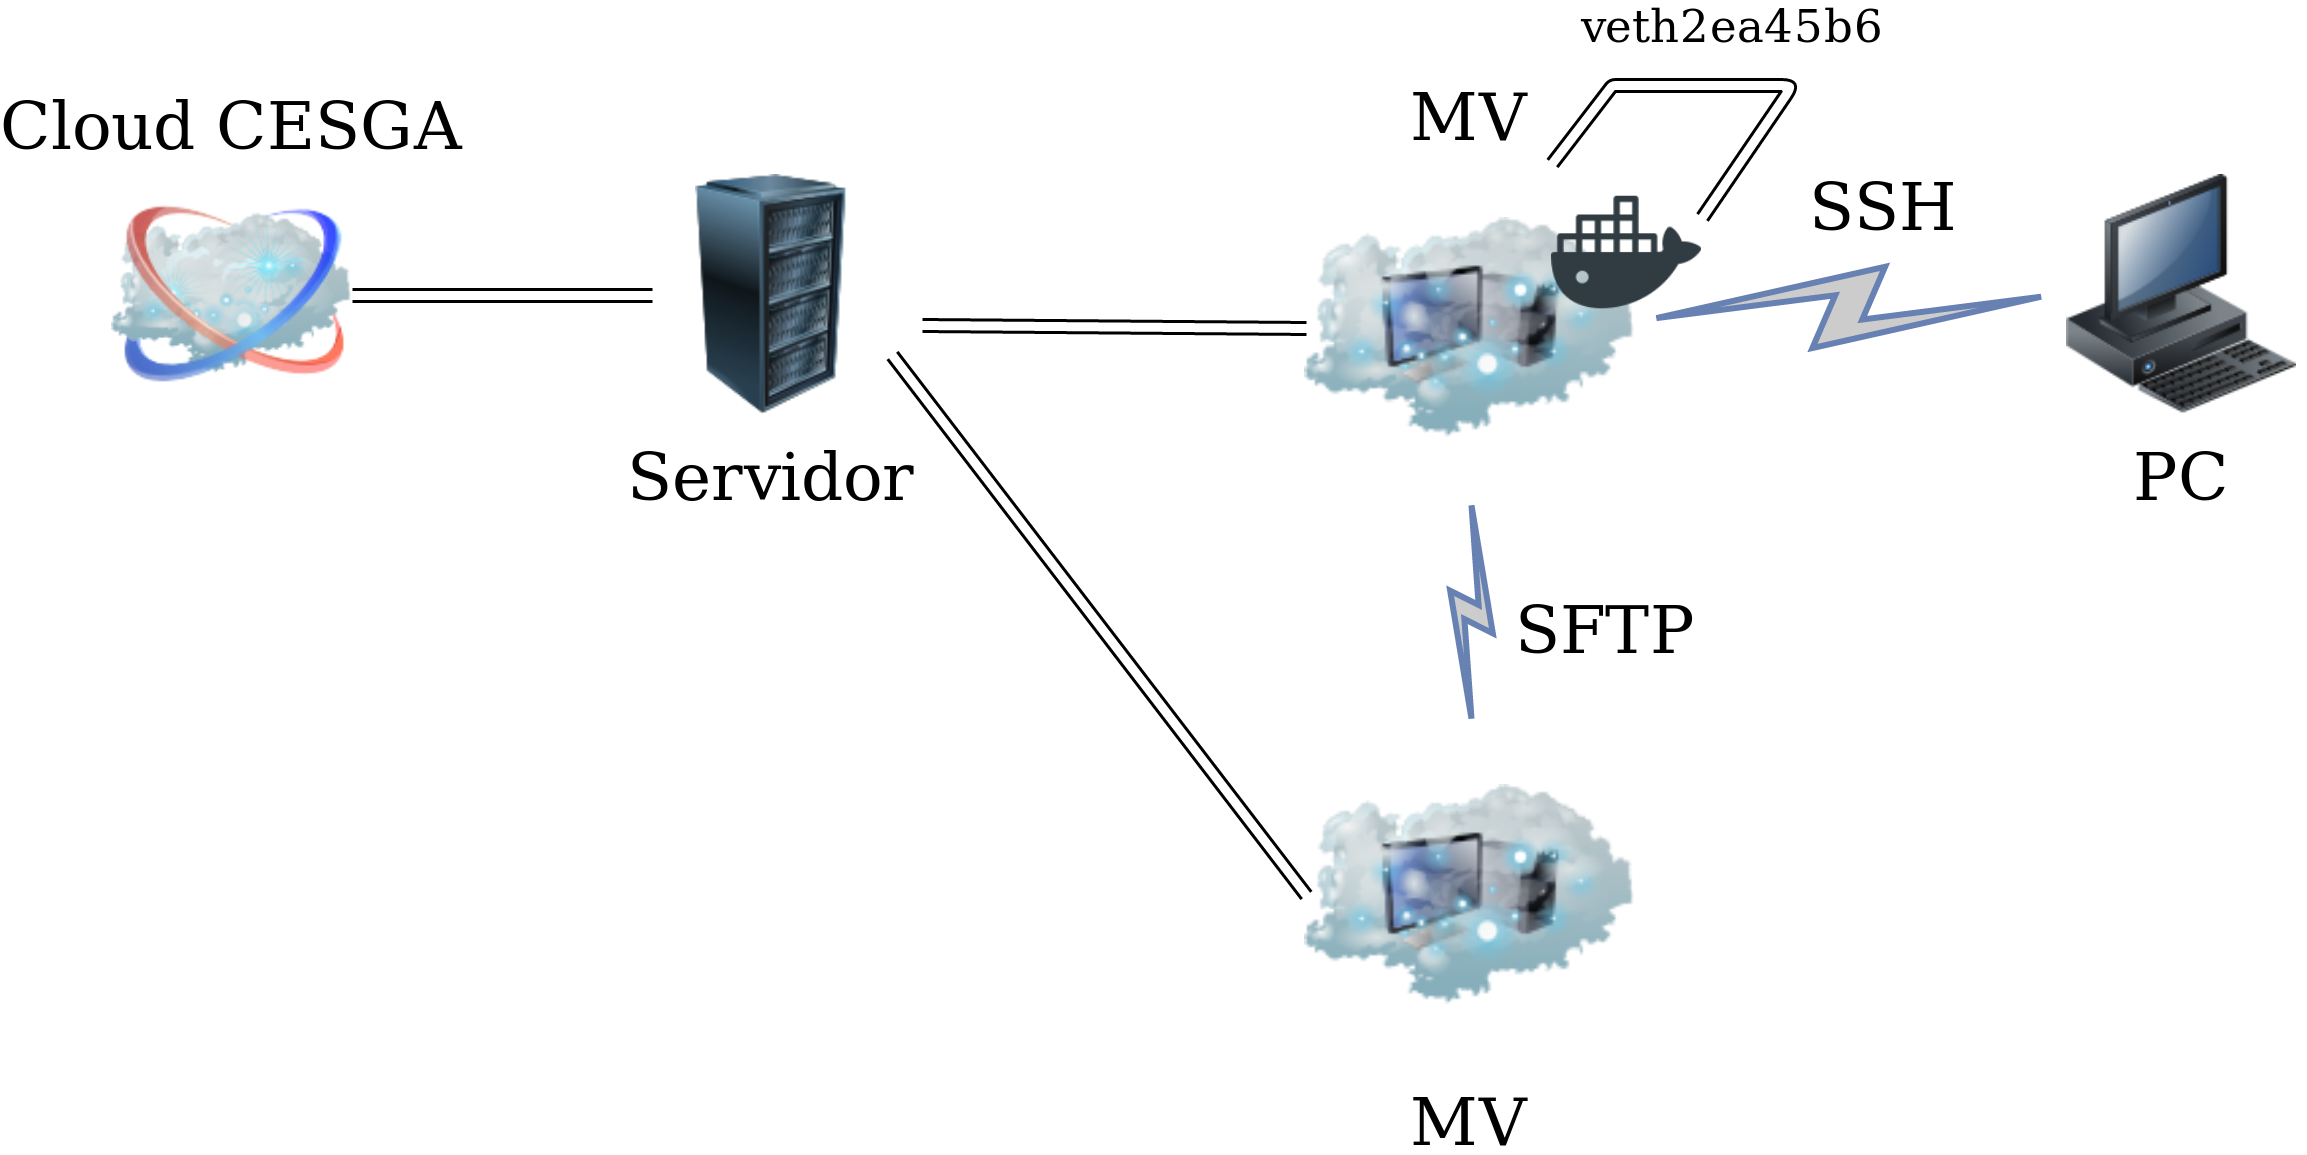
\includegraphics[width=15cm]{figuras/DiagramaQoSRedeDocker.png}}
\caption{Estrutura do despregue da QoS da rede con contedores Docker}
\label{DiagramaQoSRedeDocker}
\end{figure}

Para a realización da proba, efectuouse o envío do arquivo nun primeiro intre sen limitación algunha e logo con limitacións sobre a interface de rede do contedor empregado.\\

\begin{lstlisting}[,caption={Envío SFTP sen limitacións}]
sftp> put photo.jpg 
Uploading photo.jpg to /home/user1/photo.jpg
photo.jpg                                100% 6109KB   6.0MB/s   00:00 
\end{lstlisting}

\begin{lstlisting}[,caption={Envío SFTP con limitacións sobre o interface \textit{bridge} de Docker}]
sftp> put photo.jpg
Uploading photo.jpg to /home/user1/photo.jpg
photo.jpg                               15%  960KB   0.0KB/s - stalled -
\end{lstlisting}

Realizadas as probas pódese ver como, unha vez aplicadas as limitacións de rede, o tráfico saínte excede o máximo permitido e a transferencia non pode ser, por tanto, completada. É dicir, as limitacións aplicáronse correctamente.

\subsubsection{Probas de limitación de rede con Singularity}

No caso dos contedores Singularity, o sistema de rede empregado é o da propia máquina anfitrioa, polo que para poder aplicar limitacións farémolo sobre usuarios concretos. Deste xeito, o conxunto de contedores lanzados por un usuario soamente poderán empregar unhas características reducidas da rede segundo o criterio que o administrador de rede desexe seguir.\\

Para facer unha aproximación práctica das limitacións de rede que se queren acadar, realizarase unha proba de concepto na que se limitará a velocidade do tráfico de saída de certos usuarios.\\

Concretamente, na proba a realizar, axuntarase unha disciplina de cola directamente á raíz ({\it root}) do dispositivo. A disciplina a empregar será {\it prio}, unha disciplina moi simple que contén un número arbitrario de clases con distinta prioridade. Posto que se trata dunha proba de concepto e non dun caso real, con dúas clases bastaríanos; mais o número de clases mínimo permitido é tres. Estas clases serán creadas automaticamente, ao establecer a disciplina {\it prio}, polo que non fará falla crealas explicitamente. Ademais, a estas clases seranlle establecidas unhas disciplinas de colas sen clases (\textit{qdisc} secundarias) para marcar filtros, neste caso baseados en marcas colocadas mediante \textit{iptables}. Estas últimas disciplinas foron de tipo {\it tbf}, as cales deixan pasar paquetes até unha determinada taxa, pero coa posibilidade de aceptar refachos curtos que excedan ese límite. No referente ás limitacións establecidas, as colas terán un máximo de 1514 bytes e o tamaño dos refachos será de 1514 tamén. Para un dos usuarios limitados establecerase  unha taxa de saída de 40 kbps e para o segundo, 10 kbps. O esquema seguido pode ser apreciado na figura \ref{qdiscSingularity}, e o código asociado, no apéndice \ref{scriptQoSSingularity}. \\

\begin{figure}
\centerline{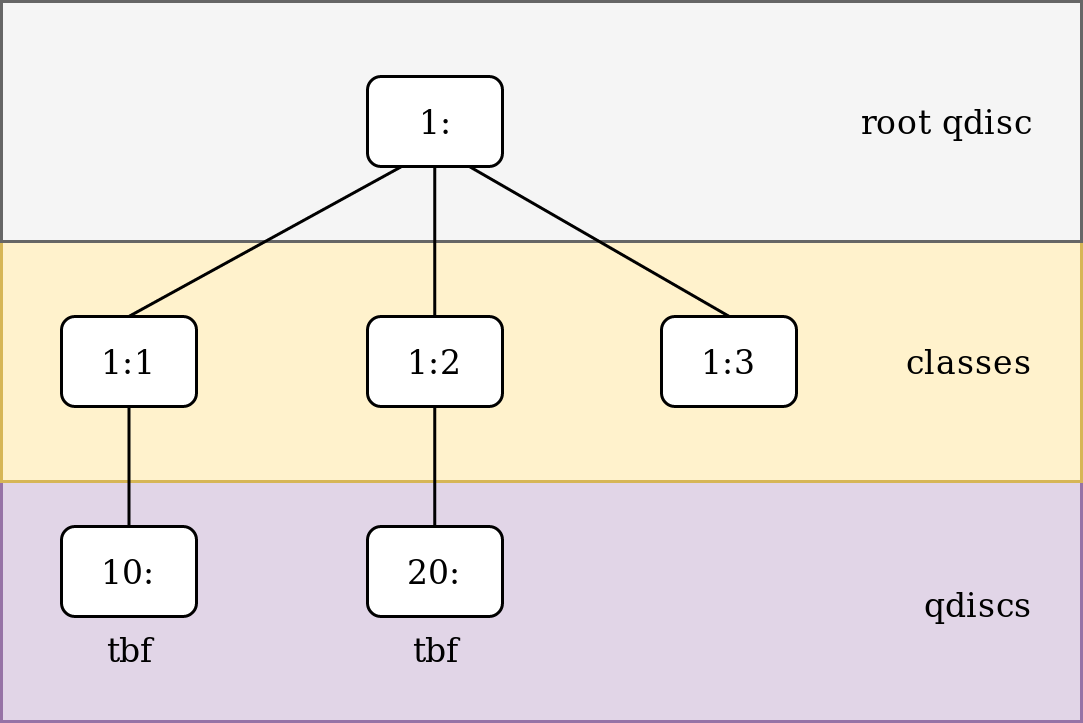
\includegraphics[width=15cm]{figuras/qdiscSingularity.png}}
\caption{Esquema da QoS da rede mediante {\it tc} en contedores Singularity}
\label{qdiscSingularity}
\end{figure}

Unha vez acadado o proceso a seguir para establecer as limitacións externas da rede segundo unha diferenciación mediante usuarios, realizouse a proba pertinente. Despegáronse dúas máquinas virtuais sobre o servizo de computación na nube do \gls{CESGA} correndo Ubuntu Xenial 16.04. Sobre unha destas máquinas aplicáronse as regras dadas no código do apéndice \ref{scriptQoSSingularity} e instalouse a tecnoloxía de contedorización Singularity. Aplicadas as limitacións pertinentes, efectuouse unha conexión \gls{SFTP} cara a segunda máquina virtual despregada, e procedeuse á transferencia dun arquivo de 5MB, coa que foi posíbel visualizar o correcto establecemento dos límites. O esquema da estrutura despregada pode ser observado na figura \ref{DiagramaQoSRedeSingularity}.\\

\begin{figure}
\centerline{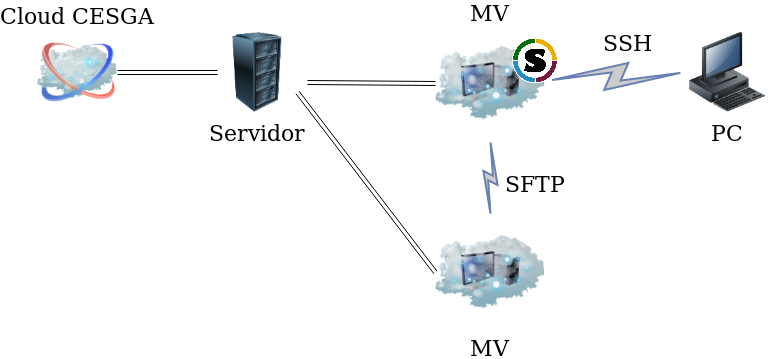
\includegraphics[width=15cm]{figuras/DiagramaQoSRedeSingularity.png}}
\caption{Estrutura do despregue da QoS da rede con contedores Singularity}
\label{DiagramaQoSRedeSingularity}
\end{figure}

A proba da transferencia realizouse como superusuario, o cal non tiña ningunha restrición, e como \textit{user1}, o cal si posuía un límite dado. Realizada a proba, as diferenzas e limitacións quedaron demostradas.

\begin{lstlisting}[,caption={Envío SFTP como superusurio}]
root@localhost:/home# singularity shell ubuntu_latest.img 
Singularity: Invoking an interactive shell within container...

Singularity ubuntu_latest.img:/home> sftp user2@10.38.3.5
user2@10.38.3.5's password: 
Connected to 10.38.3.5.
sftp> put photo.jpg 
Uploading photo.jpg to /home/user2/photo.jpg
photo.jpg                                100% 5082KB   5.0MB/s   00:00    
\end{lstlisting}

\begin{lstlisting}[,caption={Envío SFTP como \textit{user1}}]
user1@localhost:/home$ singularity shell ubuntu_latest.img
Singularity: Invoking an interactive shell within container...

Singularity ubuntu_latest.img:/home> sftp user2@10.38.3.5
user2@10.38.3.5's password: 
Connected to 10.38.3.5.
sftp> put photo.jpg 
Uploading photo.jpg to /home/user2/photo.jpg
photo.jpg                                100% 5082KB   3.9KB/s   21:38
\end{lstlisting}

Como se pode apreciar, a transferencia efectuada como superusuario realizouse coa maior celeridade posíbel, enviándose de forma practicamente instantánea. Porén, cando repetimos o envío como o usuario \textit{user1}, pódese ver como as limitacións entran en xogo e esta tarda numerosos minutos en completarse, presentando unha taxa de transferencia incluso menor á indicada.
